\section{Feature selection and dimensionality reduction}
\label{sec:feature-selection}

\emph{Writing prompt: compare all features, ANOVA selection, PCA and LDA in one
compact table. Explain constant-feature removal, F-score ranking versus selected
feature count, variance preservation versus class separation, and interpretability.
List ANOVA counts 25/50/100, PCA 10/40/95\% variance and the binary-task LDA limit
of one component. Explain why ANOVA 150 was invalid at 115--116 available columns.}

\begin{figure}[htbp]
    \centering
    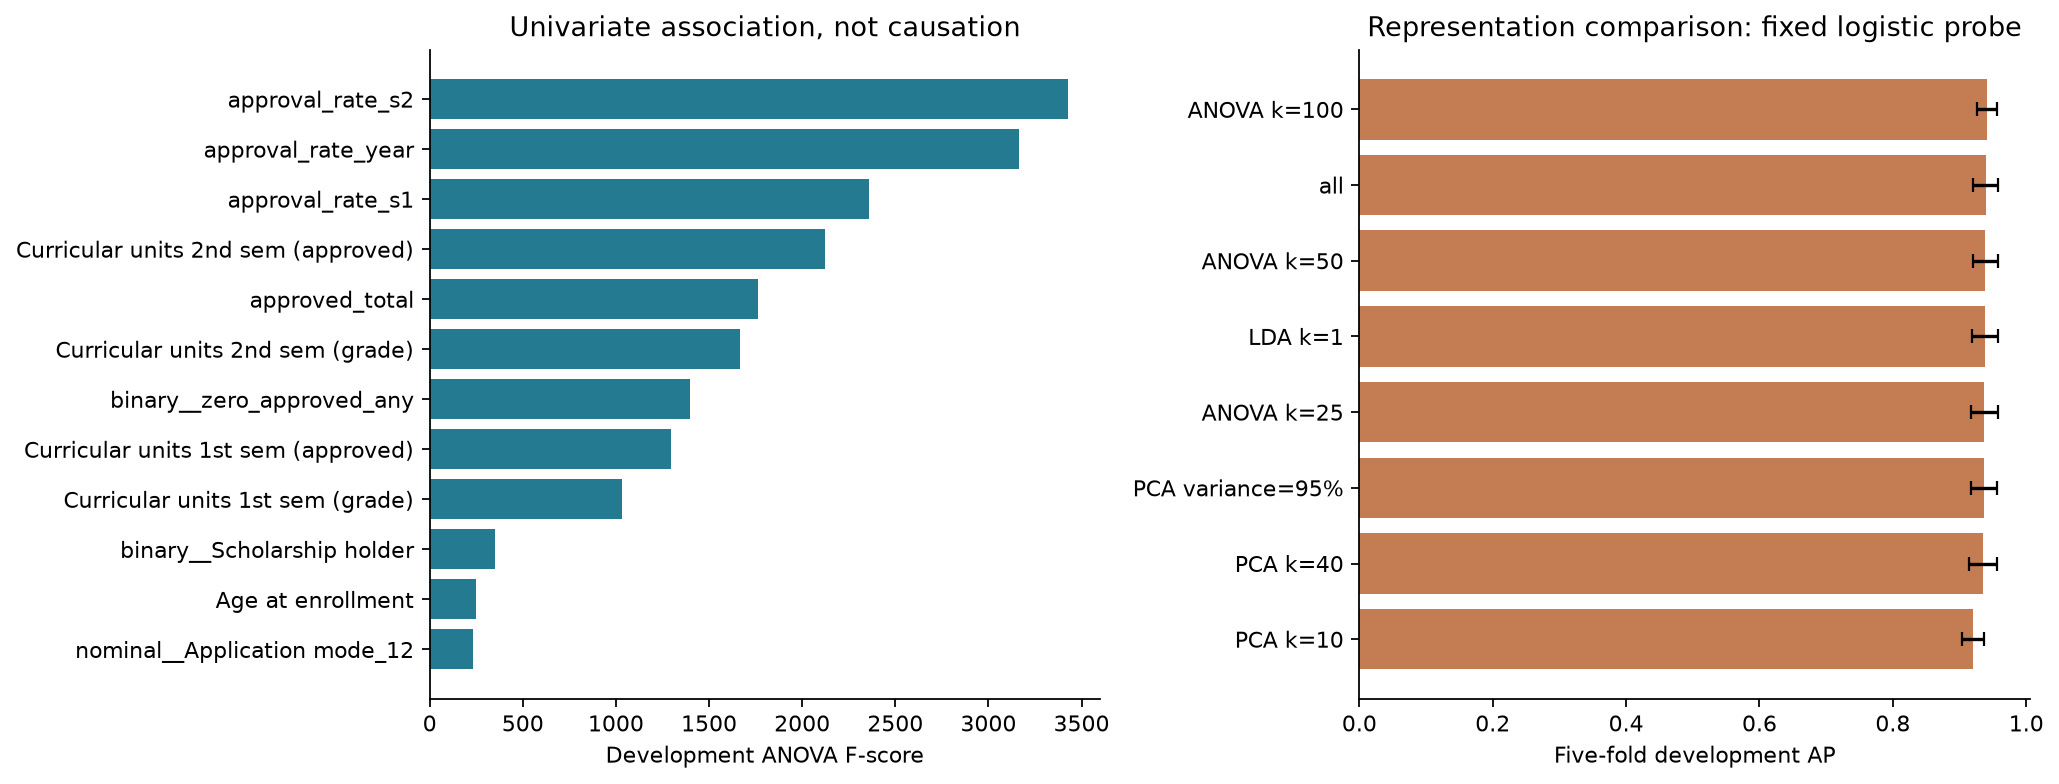
\includegraphics[width=\linewidth]{Images/01_features_and_representations.png}
    \caption{Training feature ranking and development representation comparison
    with a fixed logistic-regression probe; error bars show fold standard deviation.}
    \label{fig:feature-representations}
\end{figure}

\emph{Writing prompt: interpret the probe comparison without treating it as a
universal ranking. Representations are also tuned jointly with each classifier;
report those choices in Section~\ref{sec:classification-algorithms}.}

% Evidence: representation_probe.csv, development_anova_ranking.csv,
% inputs_KNN.csv, inputs_Decision_tree.csv and inputs_SVM.csv.
